\documentclass[list, windows]{BHCexam}
\usepackage{tikz}
\usepackage{amsmath}
\usetikzlibrary{positioning, calc, shapes.geometric, shapes, shapes.multipart, arrows.meta, arrows, decorations.markings, external, trees}
\pagestyle{fancy}
\fancyfoot[C]{第 \thepage 页 共 \pageref{lastpage} 页}
%\fancyhead[L]{\includegraphics[width=2cm]{qrcode.png}}
%\fancyhead[R]{\raisebox{0.5\height}{\includegraphics[height=1cm]{logo.png}}}
\begin{document}
\tikzstyle{Arrow} = [
thick,
decoration={
	markings,
	mark=at position 1 with {
	\arrow[thick]{latex}
	}
},
shorten >= 3pt, preaction = {decorate}
					]
\title{华东师范大学期中试卷}
\subtitle{2022-2023学年第2学期}
%\notice{\emph{考生注意:}\\1.本场考试时间90分钟,试卷共5页,满分100分,答题纸共2页.\\
%2.作答前,在答题纸正面填写姓名、准考证号,反面填写姓名.将核对后的条形码黏贴在答题纸上.\\
%3.所有作答必须填涂或书写在答题纸上与试卷题号相对应的区域,不得错位,在试卷上作答一律不得分.\\
%4.用2B铅笔作答选择题,用黑色签字笔、水笔或圆珠笔作答非选择题.}
\author{
课程名称:\underline{数据科学与工程算法}	课程性质:\underline{专业必修}\\
专业:\underline{~~~~~~~~~~~~~~~~~~~~~~~~~~}	年级:\underline{~~~~~~~~~~~~~~~~~~~~~~~~~~}	\\
姓名:\underline{~~~~~~~~~~~~~~~~~~~~~~~~~~}	学号:\underline{~~~~~~~~~~~~~~~~~~~~~~~~~~}	
}
\date{......................................................................................................................................................................}
\maketitle
\begin{center}
    \begin{tabular}{| l | l | l | l | l | l | l |}
    \hline
	/& 一 & 二 & 三 & 四 & 五 & 总分 \\ \hline
    得分 & ~ & ~ & ~ & ~ & ~ & ~\\ \hline
    \end{tabular}
\end{center}
\begin{groups}
\group{填空题}{(本大题共有8题,满分48分,每题6分.)}

\begin{questions}[p]
\begin{minipage}{\linewidth}
\question [4] 采用圆形等距抽样算法从总体$1$-$21$中抽取样本.抽样间距为$4$,第一个被抽样的元素编号为$15$,请问接下去被抽样的四个元素编号依次是\key{$15,19,2,6$}.

\end{minipage}
\begin{solution}{4cm}

\end{solution}
%\vfill
\begin{minipage}{\linewidth}
\question [4] 假设抛一枚正面向上概率为$\frac{3}{4}$的硬币$1000$次,随机变量$X$定义为硬币正面朝上的次数,使用Chebyshev不等式估算$X>900$的概率上界为\key{$\frac{1}{120}$}.

\end{minipage}
\begin{solution}{4cm}

\end{solution}
%\vfill
\begin{minipage}{\linewidth}
\question [4] 假设抛一枚正面向上概率为$\frac{1}{5}$的硬币$800$次,随机变量$X$定义为硬币正面朝上的次数,使用Chernoff不等式估算$X<40$的概率上界为\key{$e^{-45}$}.

\end{minipage}
\begin{solution}{4cm}

\end{solution}
%\vfill
\begin{minipage}{\linewidth}
\question [4] 当哈希函数$h(x)=(3x+1)mod 5$被用于行排列变换时,集合$A=\{0,1,4\}$和$B=\{2,3,4\}$的最小哈希值分别为\key{$1,0$}.

\end{minipage}
\begin{solution}{4cm}

\end{solution}
%\vfill
\begin{minipage}{\linewidth}
\question [4] 设$k=3$,使用Misra Gries算法求得输入数据流$<a,b,b,c,c,a,a,d>$中的频繁元素为\key{a,d}.

\end{minipage}
\begin{solution}{4cm}

\end{solution}
%\vfill
\begin{minipage}{\linewidth}
\question [4] 对于输入数据流$<0,1,1,2,3,3>$,假设给定哈希函数$h_{1}(x)=(2x+1) mod 3$和$h_{2}(x)=(x+1) mod 3$,用CM Sketch估计元素$0$的频度为\key{$3$}.

\end{minipage}
\begin{solution}{4cm}

\end{solution}
%\vfill
\begin{minipage}{\linewidth}
\question [4] 对于数据流$<0,0,1,2,2,3,3,3>$,假设给定哈希函数$h(x)=(7x+2) mod 3$和
$g(x) =
\begin{cases}
+1 &\quad\text{if x mod 2 = 0}\\
-1 &\quad\text{if x mod 2 = 1}\\
\end{cases}$,用Count Sketch估计元素$1$的频度为\key{$1$}.

\end{minipage}
\begin{solution}{4cm}

\end{solution}
%\vfill
\begin{minipage}{\linewidth}
\question [4] 对于转移概率矩阵为
$ 
\mathbf{P}=      %开始数学环境
\left(                 %左括号
  \begin{array}{ccc}   %该矩阵一共3列,每一列都居中放置
    \frac{1}{2} & \frac{1}{4} & \frac{1}{4}\\  %第一行元素
    0 & \frac{1}{4} & \frac{3}{4}\\  %第二行元素
	p & 1-p & 0\\
  \end{array}
\right)                 %右括号
$的马尔可夫链,已知其平稳分布为$(\frac{1}{3},\frac{1}{3},\frac{1}{3})$,则参数$p$的取值是\key{$\frac{1}{2}$}.

\end{minipage}
\begin{solution}{4cm}

\end{solution}

\end{questions}
\newpage
\group{}{(本题满分20分,其中每题10分.)}

\begin{questions}[p]
\begin{minipage}{\linewidth}
\question [20] 设一组独立随机变量$x_{ij}(i = 1,......,k;j=1,......,n)$服从参数为$p$的伯努利分布.定义随机变量$X_{i}=\frac{1}{n}\sum_{j=1}^{n}x_{ij},i = 1,......,k$.
\begin{subquestions}
	\subquestion 设随机变量$Y = min_{1\leq i\leq k}X_{i}$,计算事件$Y>(1+\epsilon)p$的概率上界;
	\subquestion 设随机变量$Z = median_{1\leq i\leq k}X_{i}$,计算事件$|Z-p|>\epsilon p$的概率上界.
\end{subquestions}
\end{minipage}
\begin{solution}{4cm}

\end{solution}
\end{questions}
\group{}{(本题满分12分.)}

\begin{questions}[p]
\begin{minipage}{\linewidth}
\question [12] 给定两个集合$A$,$B$各包含$50$亿个元素,每个元素占用$64B$。当内存使用被限制在$4\times10^9B$时,设计怡当的方案计算集合$A$和$B$的交集,并分析方案的误差.
\end{minipage}
\begin{solution}{4cm}

\end{solution}
\end{questions}

\group{}{(本题满分10分.)}

\begin{questions}[p]
\begin{minipage}{\linewidth}
\question [10] 若存在四个网站$A$、$B$、$C$、$D$,其链接关系如图所示.使用随机跳转参数$p=0.2$的改进版PageRank算法计算每个网站的PageRank值.
\end{minipage}
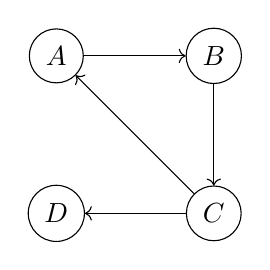
\begin{tikzpicture}
\node[circle,
minimum width =5pt ,
minimum height =5pt ,draw=black] (1) at(0,2){$A$};
\node[circle,
minimum width =5pt ,
minimum height =5pt ,draw=black] (2) at(2,2){$B$};
\node[circle,
minimum width =5pt ,
minimum height =5pt ,draw=black] (3) at(0,0){$D$};
\node[circle,
minimum width =5pt ,
minimum height =5pt ,draw=black] (4) at(2,0){$C$};
\draw[->] (1) --(2);
\draw[->] (2) --(4);
\draw[->] (4) --(1);
\draw[->] (4) --(3);
\end{tikzpicture}
\begin{solution}{4cm}

\end{solution}
\end{questions}

\group{}{(本题满分10分.)}

\begin{questions}[p]
\begin{minipage}{\linewidth}
\question [10] 使用Flajolet-Martin算法估算数据流$<3,1,4,1,8,2,9>$中不同元素的个数,使用哈希函数$h_{1}(x) = (2x+1)mod 16$和$h_{2}(x)=(4x) mod 16$.请给出算法运行结果.
\end{minipage}
\begin{solution}{4cm}

\end{solution}
\end{questions}

\end{groups}
\label{lastpage}
\end{document}
